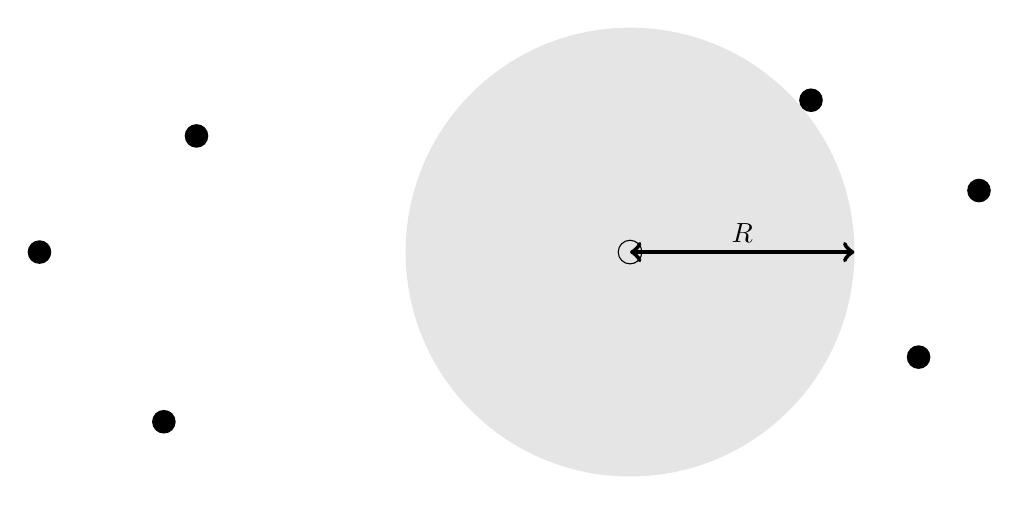
\begin{tikzpicture}[scale=3]
% Parameters
\def\radius{1};
\def\validR{0.95};
\def\sourceR{1-\validR}

\pgfmathsetmacro\evalX{cos(140)*\radius}
\pgfmathsetmacro\evalY{sin(140)*\radius}

\pgfmathsetmacro\sourceXa{cos(-20)*1.3*\radius}
\pgfmathsetmacro\sourceYa{sin(-20)*1.3*\radius}

\pgfmathsetmacro\sourceXb{cos(10)*1.5*\radius}
\pgfmathsetmacro\sourceYb{sin(10)*1.5*\radius}

\pgfmathsetmacro\sourceXc{cos(200)*2.1*\radius}
\pgfmathsetmacro\sourceYc{sin(200)*2.1*\radius}

\pgfmathsetmacro\sourceXd{cos(180)*2.5*\radius}
\pgfmathsetmacro\sourceYd{sin(180)*2.5*\radius}

\pgfmathsetmacro\sourceXe{cos(165)*1.9*\radius}
\pgfmathsetmacro\sourceYe{sin(165)*1.9*\radius}

\pgfmathsetmacro\sourceXf{cos(40)*\radius}
\pgfmathsetmacro\sourceYf{sin(40)*\radius}

\fill [color=black,opacity=0.1] (0,0) circle (\validR*\radius);

%\node at (0,0){$\times$};
\draw [color=black] (0,0) circle (\sourceR*\radius);
\draw[ultra thick,<->] (0,0) -- (\validR*\radius,0);
\node[above] at (0.5*\validR*\radius,0){$R$};

% Source positions
\fill [color=black] (\sourceXa,\sourceYa) circle (\sourceR*\radius);
\fill [color=black] (\sourceXb,\sourceYb) circle (\sourceR*\radius);
\fill [color=black] (\sourceXc,\sourceYc) circle (\sourceR*\radius);
\fill [color=black] (\sourceXd,\sourceYd) circle (\sourceR*\radius);
\fill [color=black] (\sourceXe,\sourceYe) circle (\sourceR*\radius);
\fill [color=black] (\sourceXf,\sourceYf) circle (\sourceR*\radius);
\end{tikzpicture}